\documentclass[tikz,border=5pt]{standalone}
\usepackage{tikz}
\usepackage{amsmath,amssymb}
\usetikzlibrary{positioning,arrows.meta,fit,calc,backgrounds}

%% ── Palette ──────────────────────────────────────────────────────────────────
\definecolor{corecol}{RGB}{41,98,178}
\definecolor{corelite}{RGB}{218,228,252}
\definecolor{optcol}{RGB}{60,60,60}

\begin{document}
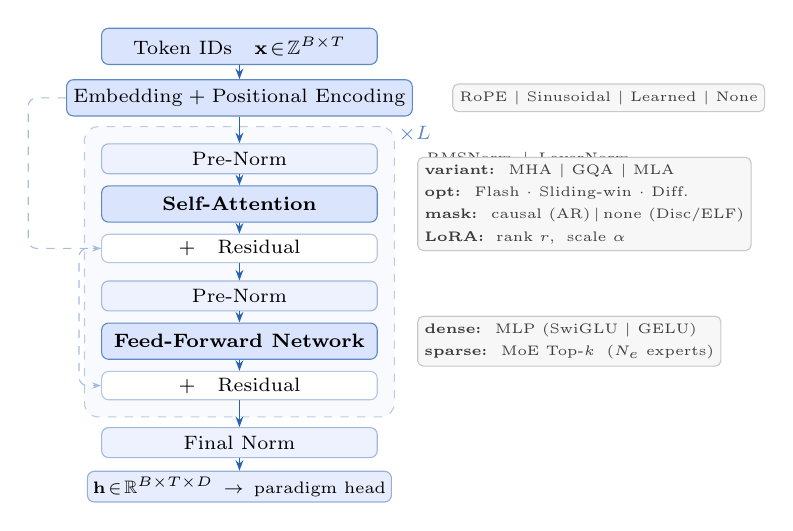
\begin{tikzpicture}[
  every node/.style={font=\scriptsize},
  %% main block — vivid blue fill
  mb/.style={
    draw=corecol!75, fill=corelite,
    rounded corners=2.5pt,
    minimum width=3.50cm, minimum height=0.46cm,
    align=center, inner sep=2.5pt
  },
  %% normalisation sublayer — lighter shade
  nm/.style={
    draw=corecol!45, fill=corelite!48,
    rounded corners=2.5pt,
    minimum width=3.50cm, minimum height=0.38cm,
    align=center, inner sep=2pt
  },
  %% residual addition node — white interior so it reads as a junction
  ra/.style={
    draw=corecol!35, fill=white,
    rounded corners=2.5pt,
    minimum width=3.50cm, minimum height=0.36cm,
    align=center, inner sep=2pt
  },
  %% annotation box on the right
  ob/.style={
    draw=optcol!28, fill=optcol!4,
    rounded corners=2pt,
    font=\fontsize{5.5}{6.5}\selectfont,
    text=optcol,
    align=left, inner sep=2.5pt
  },
  %% main forward arrows
  arr/.style={-{Stealth[length=3.8pt,width=2.8pt]}, semithick, corecol},
  %% dashed residual skip connections
  sk/.style={
    -{Stealth[length=3.2pt,width=2.3pt]},
    dashed, corecol!42,
    rounded corners=3pt, thin
  },
]

%%── Input token IDs ──────────────────────────────────────────────────────────
\node[mb] (tok)
  {Token IDs\quad$\mathbf{x}\!\in\!\mathbb{Z}^{B\times T}$};

%%── Token embedding + positional encoding ────────────────────────────────────
\node[mb, below=0.18cm of tok] (emb)
  {Embedding\;+\;Positional Encoding};
\node[ob, right=0.50cm of emb, anchor=west] (embo)
  {RoPE \textbar{} Sinusoidal \textbar{} Learned \textbar{} None};

%%── Transformer Block  (×L) ──────────────────────────────────────────────────

\node[nm, below=0.34cm of emb] (pn1)
  {Pre-Norm};
\node[font=\fontsize{5}{6}\selectfont, optcol,
      right=0.50cm of pn1, anchor=west] (pn1a)
  {RMSNorm \,\textbar\, LayerNorm};

\node[mb, below=0.14cm of pn1] (attn)
  {\textbf{Self-Attention}};
\node[ob, right=0.50cm of attn, anchor=west] (attno)
  {\textbf{variant:}\; MHA \textbar{} GQA \textbar{} MLA\\[1.5pt]
   \textbf{opt:}\; Flash $\cdot$ Sliding-win $\cdot$ Diff.\\[1.5pt]
   \textbf{mask:}\; causal (AR)\,\textbar\,none (Disc/ELF)\\[1.5pt]
   \textbf{LoRA:}\; rank $r$,\; scale $\alpha$};

\node[ra, below=0.14cm of attn] (res1)
  {$+$\quad Residual};

\node[nm, below=0.22cm of res1] (pn2)
  {Pre-Norm};

\node[mb, below=0.14cm of pn2] (ffn)
  {\textbf{Feed-Forward Network}};
\node[ob, right=0.50cm of ffn, anchor=west] (ffno)
  {\textbf{dense:}\; MLP (SwiGLU \textbar{} GELU)\\[1.5pt]
   \textbf{sparse:}\; MoE Top-$k$\; ($N_e$ experts)};

\node[ra, below=0.14cm of ffn] (res2)
  {$+$\quad Residual};

%%── Dashed frame around the repeated block ───────────────────────────────────
\begin{pgfonlayer}{background}
  \node[draw=corecol!32, dashed, fill=corecol!3,
        rounded corners=5pt,
        fit=(pn1)(res2),
        inner sep=6pt] (blk) {};
\end{pgfonlayer}

%% ×L badge at top-right corner of the frame
\node[font=\scriptsize\bfseries, text=corecol!75,
      anchor=north west, inner sep=0pt]
  at ($(blk.north east)+(0.04cm,0)$)
  {$\times L$};

%%── Final normalisation and output ───────────────────────────────────────────
\node[nm, below=0.34cm of res2] (fnorm)
  {Final Norm};

\node[draw=corecol!50, fill=corelite!65,
      rounded corners=2.5pt,
      minimum width=3.50cm, minimum height=0.38cm,
      align=center, inner sep=2pt,
      font=\fontsize{6.5}{7.5}\selectfont,
      below=0.16cm of fnorm] (outp)
  {$\mathbf{h}\!\in\!\mathbb{R}^{B\times T\times D}$\enspace
   $\to$\enspace paradigm head};

%%── Forward arrows ───────────────────────────────────────────────────────────
\foreach \s/\t in
  {tok/emb, emb/pn1, pn1/attn, attn/res1,
   res1/pn2, pn2/ffn, ffn/res2, res2/fnorm, fnorm/outp}
  \draw[arr] (\s) -- (\t);

%%── Residual skip connections (drawn on the left) ────────────────────────────
%% Skip 1: block input (= emb output)  →  add₁ (res1)
%%   Implements  x' = x + Attn(Norm(x))
\draw[sk] (emb.west) -- ++(-0.48cm,0) |- (res1.west);

%% Skip 2: add₁ output (res1)  →  add₂ (res2)
%%   Implements  x'' = x' + FFN(Norm(x'))
\draw[sk] (res1.west) -- ++(-0.28cm,0) |- (res2.west);

\end{tikzpicture}
\end{document}
